% !TEX root =path to root.tex
\documentclass[a4paper,12pt]{report} % "report" è ottimo per tesi, include chapter

\usepackage[utf8]{inputenc}          % Supporta caratteri con accenti
\usepackage[italian]{babel}
\usepackage{amsmath, amssymb}         % Pacchetti per la matematica avanzata
\usepackage{graphicx}                 % Per inserire immagini
\usepackage{hyperref}                 % Per link interni
\usepackage{geometry}                 % Imposta margini del documento

\geometry{left=3cm, right=3cm, top=3cm, bottom=3cm}

\begin{document}

\title{Studio sul Gioco del Domino}
\author{Alex Lorenzato}
\maketitle

\tableofcontents % Crea automaticamente un indice dei contenuti

\chapter{Introduzione}

\section{Il Domino}

Il domino è un antico gioco da tavolo, le cui origini risalgono alla Cina imperiale. Le tessere di gioco sono rettangolari e suddivise in due metà; su ciascuna metà è presente un valore numerico che varia tra 0 e 6, rappresentato tipicamente con dei pallini, o "pip", simili a quelli presenti sui dadi che indicano il punteggio della tessera. Le tessere formano una combinazione unica di numeri, con 28 tessere totali in un set "double-six", ovvero la cui tessere di maggior valore è quella in cui appaiono due 6.

L'obiettivo generale del gioco, sebbene esistano diverse varianti, è di liberarsi di quante più tessere possibili dalla propria mano prima della fine della partita. Il gioco procede a turni in senso orario: ogni giocatore, al suo turno, ha la possibilità di aggiungere una tessera dalla propria mano all'inizio o alla fine della sequenza di tessere presenti sul tavolo, rispettando la condizione che il valore su una delle estremità della tessera coincida con il valore della tessera a cui si collega. 

Nella variante classica, la partita inizia con il giocatore che possiede la tessera doppia con il valore più alto, di conseguenza il doppio-6 è la tessera che garantisce di partire per primi. Questa versione è particolarmente popolare nella modalità a 2 giocatori, ma può essere giocata anche da un massimo di 4 o 6 giocatori, con regole e adattamenti per gestire il numero di tessere e i turni.

\section{Storia del Domino}

Il domino con tessere nacque in Cina intorno al XII secolo e si ritiene che sia stato sviluppato da uno statista nel 1120, come dono per l'imperatore Hui Tsung. Inizialmente, il domino aveva anche un ruolo come strumento di divinazione intorno al XIII secolo, diventando poi un gioco da tavolo vero e proprio.

Nel corso del tempo, il gioco del domino si diffuse dal continente asiatico all'Europa, probabilmente grazie agli scambi culturali mediati dal mondo arabo. Giunto in Italia, il gioco si diffuse rapidamente in Francia e successivamente in tutta Europa. Il termine "domino" deriva dal latino \textit{dominus}, che significa "padrone", e sembra essere legato al senso di controllo e strategia che il gioco richiede.\footnote{Fonte: Wikipedia, "Domino", https://it.wikipedia.org/wiki/Domino (accesso il 25 ottobre 2024).}

\section{Variante "Block"}

La variante "Block" è la versione del domino utilizzata come oggetto di studio in questa tesi, nonché la variante più diffusa e popolare.

Questa versione utilizza un set di tessere "double-six", ovvero tessere con valori che vanno da 0 a 6 su ciascuna metà. Ogni giocatore pesca sette tessere all'inizio del gioco, e le rimanenti 14 tessere vengono scartate e non utilizzate per tutta la durata della partita. La partita termina in due casi:

\begin{enumerate}
    \item Quando un giocatore riesce a liberarsi di tutte le tessere in mano, vincendo automaticamente.
    \item Quando la partita è "bloccata", ossia nessuno dei due giocatori può posizionare una tessera valida.
\end{enumerate}

In caso di "blocco", vince il giocatore con il minor punteggio totale in mano, dove il punteggio è calcolato come la somma dei valori presenti sulle tessere rimanenti. Se un giocatore riesce a esaurire tutte le sue tessere, è dichiarato automaticamente vincitore.


\section{Altre varianti}

Assieme alla variante "Block", esiste la variante "Draw", che differisce per l'uso delle tessere non distribuite ai giocatori. Mentre nella "Block" le tessere avanzate vengono rimosse definitivamente dalla partita, nella variante "Draw" i giocatori possono pescare tessere aggiuntive quando non riescono a fare una mossa valida. Le modalità di pesca variano: in alcune versioni il giocatore è obbligato a pescare fino a trovare una tessera giocabile, mentre in altre può pescare solo una tessera per turno.


Queste varianti danno origine a una vasta gamma di regole aggiuntive e variazioni del gioco. Esistono inoltre numerose versioni del domino fan-made e competitive, ognuna con modifiche più o meno significative alle regole delle varianti "Block" e "Draw". Per esempio, oltre all’obiettivo tradizionale di esaurire la propria mano, alcune modalità premiano configurazioni particolari di tessere sul tavolo, rendendo il gioco ancora più strategico e vario.


\chapter{Risultati}

\section{Statistiche Globali}

Il numero totale di configurazioni delle mani iniziali, corrispondente al numero di partite diverse giocabili nel domino è: \(137.281.098.240\), calcolato nel seguente modo:


\begin{enumerate}
    \item Possibili set da 14 tessere: \(\binom{28}{14} = 40.116.600\), ai quali bisogna sottrarre tutti i set che non contengono nessuna tessera doppia.
    \item Set che non contengono nessuna tessera doppia: \(\binom{21}{14} = 116.280\).
    \item Possibili set da 14 tessere validi per poter iniziare una partita: \(40.116.600 - 116.280 = 40.000.320\), ovvero il totale di set possibili esclusi quelli senza una tessera doppia.
    \item Ognuna delle \(40.000.320\) possibili partite è costituita da un set di 14 tile, che però possono essere distrubuite in \(\binom{14}{7} = 3432\) modi diversi tra i 2 giocatori
    \item Il numero totale di partite esistenti con un set da 28 tile e mani da 7 tile ciascuna quindi è: \(40.000.320 * 3432 = 137.281.098.240\)
\end{enumerate}

Testare l'algoritmo su tutte le possibili partite non è temporalmente possibile con gli strumenti a disposizione, questo perché supponendo una media di 70ms a partita (media calcolata sui dati raccolti) ci vorrebbero \(137.281.098.240 * 70  = 9.609.676.876.800\) ms, equivalenti a \(304.7\) anni su un sistema monoprocessore; avendo avuto a disposizione un server con 40 processori, il tempo di calcolo necessario sarebbe stato \(304 / 40 \tilde= 7.5\) anni. 

\vspace{0.5cm}

Altre statistiche raccolte:
\begin{enumerate}
    \item Durata media della partita: 71.56 ms
    \item Numero medio di foglie: 1023.36
    \item Percentuale media di foglie in cui nessun giocatore aveva esaurito le tessere: 48.13\%
\end{enumerate}

La partita con il maggior numero di foglie in assoluto, ovvero 32.172, è quella in cui i giocatori hanno le seguenti mani:

\begin{quote}
    \textbf{Mano giocatore 1:} \(0|2, 1|2, 1|5, 2|2, 2|6, 4|4, 5|6\)
\end{quote}

\begin{quote}
    \textbf{Mano giocatore 2:} \(0|4, 1|4, 1|6, 2|4, 2|5, 4|5, 4|6\) 
\end{quote}



Un'altra statistica interessante è che ci sono \( 356.142 \) partite con una sola foglia, equivalenti al \( 9\%\), questo accade perché un giocatore ha una doppia tessera con cui partire ma poi né lui né l'avversario hanno una tessera che si può attaccare a quella inizialmente giocata.


Il numero di foglie è indice della complessità della partita, con una sola foglia la partita è banale e non necessita che vengano prese decisioni, al contrario se si hanno migliaia di foglie la partita permette molta libertà d'azione e l'ordine in cui vengono giocate le tessere assume molta più importanza.


Un esempio banale di partita ad una sola foglia è dato da un giocatore che parte con la tessera doppio-6 e nessuno dei due giocatori ha altre tessere in cui compaia un 6, la partita quindi termina immediatamente procedendo al calcolo del punteggio.


Non è comunque garantito che un alto numero di foglie indichi una partita complessa, spesso si presentano dinamiche per cui l'ordine in cui vengono giocate le tessere è ininfluente ai fini del risultato finale; questo tipo di partite hanno solo una complessità apparente, ma di fatto sono banali quanto quelle con poche foglie.


\section{Statistiche di set specifici}

Ho investigato dei set specifici di tessere alla ricerca di mani più o meno vantaggiose in termini di partite vinte, i risultati sono i seguenti:


\begin{quote}
    \textbf{Mano:} \(0|0, 0|1, 0|2, 0|3, 0|4, 0|5, 0|6\)
\end{quote}

\begin{table}[h!]
    \centering
    \begin{tabular}{|l|c|}
        \hline
        Match considerati & 65 \\
        Durata media delle partite & 88.35 ms \\
        Numero medio di foglie & 2257.60 \\
        Percentuale di vittorie & 100.00\% \\
        Percentuale di partite in cui nessun giocatore esauriva la mano & 24.65\% \\
        \hline
    \end{tabular}
    \caption{Statistiche per la mano \(0|0, 0|1, 0|2, 0|3, 0|4, 0|5, 0|6\)}
    \label{tab:stats_1}
\end{table}

Questa configurazione di mano iniziale è chiaramente vantaggiosa dato sono state vinte tutte le partite affrontate.

Soffre di uno svantaggio iniziale, ovvero la difficoltà a partire per primi, visto che qualsiasi tessera doppia garantirebbe la precedenza su questa mano; superato questo difetto,
si ha una mano che riesce ad agganciarsi ad ogni tessera giocata visto che si hanno tutti i numeri da 0 a 6, inoltre è molto facile connettere le tessere tra loro usando il numero 0 come "aggancio";
un ulteriore vantaggio è quello di chiudere le possibilità all'avversario, visto che non potrà avere tessere con il numero 0 in quanto le ha tutte il giocatore con questa mano, ne segue che una delle 
due estremità del tavolo è spesso bloccata dal numero 0. 


\begin{quote}
    \textbf{Mano:} \(0|0, 1|1, 2|2, 3|3, 4|4, 5|5, 6|6\)
\end{quote}

\begin{table}[h!]
    \centering
    \begin{tabular}{|l|c|}
        \hline
        Match considerati & 64 \\
        Durata media delle partite & 43.84 ms \\
        Numero medio di foglie & 55.72 \\
        Percentuale di vittorie & 34.38\% \\
        Percentuale di partite in cui nessun giocatore esauriva la mano & 73.81\% \\
        \hline
    \end{tabular}
    \caption{Statistiche per la mano \(0|0, 1|1, 2|2, 3|3, 4|4, 5|5, 6|6\)}
    \label{tab:stats_1}
\end{table}

Ho scelto di investigare questa mano per la particolarità di avere tutte le doppie, i risultati non sono stati buoni visto che il rateo di vittoria è di 1 su 3.

Il motivo per cui questa mano non funziona bene potrebbe essere dato dal fatto che di fatto non ha possibilità di prendere decisioni significative; ogni volta che collega una tessera, il tavolo rimane invariato, di conseguenza è l'avversario che tramite delle tessere diversificate può gestire la partita in maniera autonoma, il giocatore con questa mano non può fare altro che attaccare le tessere che ha senza mai influire sulle estremità del tavolo.

Presenta solo due vantaggi, chiaramente insufficienti: garanzia di iniziare per primo e avere tutti i numeri in mano, quindi potersi attaccare facilmente ad ogni situazione, con lo svantaggio di poterlo fare una volta sola per numero.

\begin{quote}
    \textbf{Mano:} \(0|0, 0|1, 0|2, 0|3, 1|1, 1|2, 1|3\)
\end{quote}

\begin{table}[h!]
    \centering
    \begin{tabular}{|l|c|}
        \hline
        Match considerati & 69 \\
        Durata media delle partite & 75.39 ms \\
        Numero medio di foglie & 1580.77 \\
        Percentuale di vittorie & 55.07\% \\
        Percentuale di partite in cui nessun giocatore esauriva la mano & 31.81\% \\
        \hline
    \end{tabular}
    \caption{Statistiche per la mano \(0|0, 1|1, 2|2, 3|3, 4|4, 5|5, 6|6\)}
    \label{tab:stats_1}
\end{table}

Questa mano è caratterizzata da una distribuzione di tessere dai valori bassi, i risultati sono relativamente scarsi, appena al di sopra del tiro di una moneta in quanto a probabilità di vittoria.
Il potenziale di questa mano era quello di avere tessere ben connesse e coese tra loro, cercando di tagliare le possibilità all'avversario andando a creare un "circuito chiuso".
Un grosso svantaggio è quello di avere poche probabilità di iniziare per primi, andando a limitare fin dall'inizio la possibilità di creare un tavolo formato da tessere basse.

\section{Grafici}

Di seguito sono rappresentati dei grafici, il primo dei quali (figura 2.1) è quello generale, gli altri sono ingrandimenti di specifici intervalli.


\begin{figure}[h!]
    \centering
    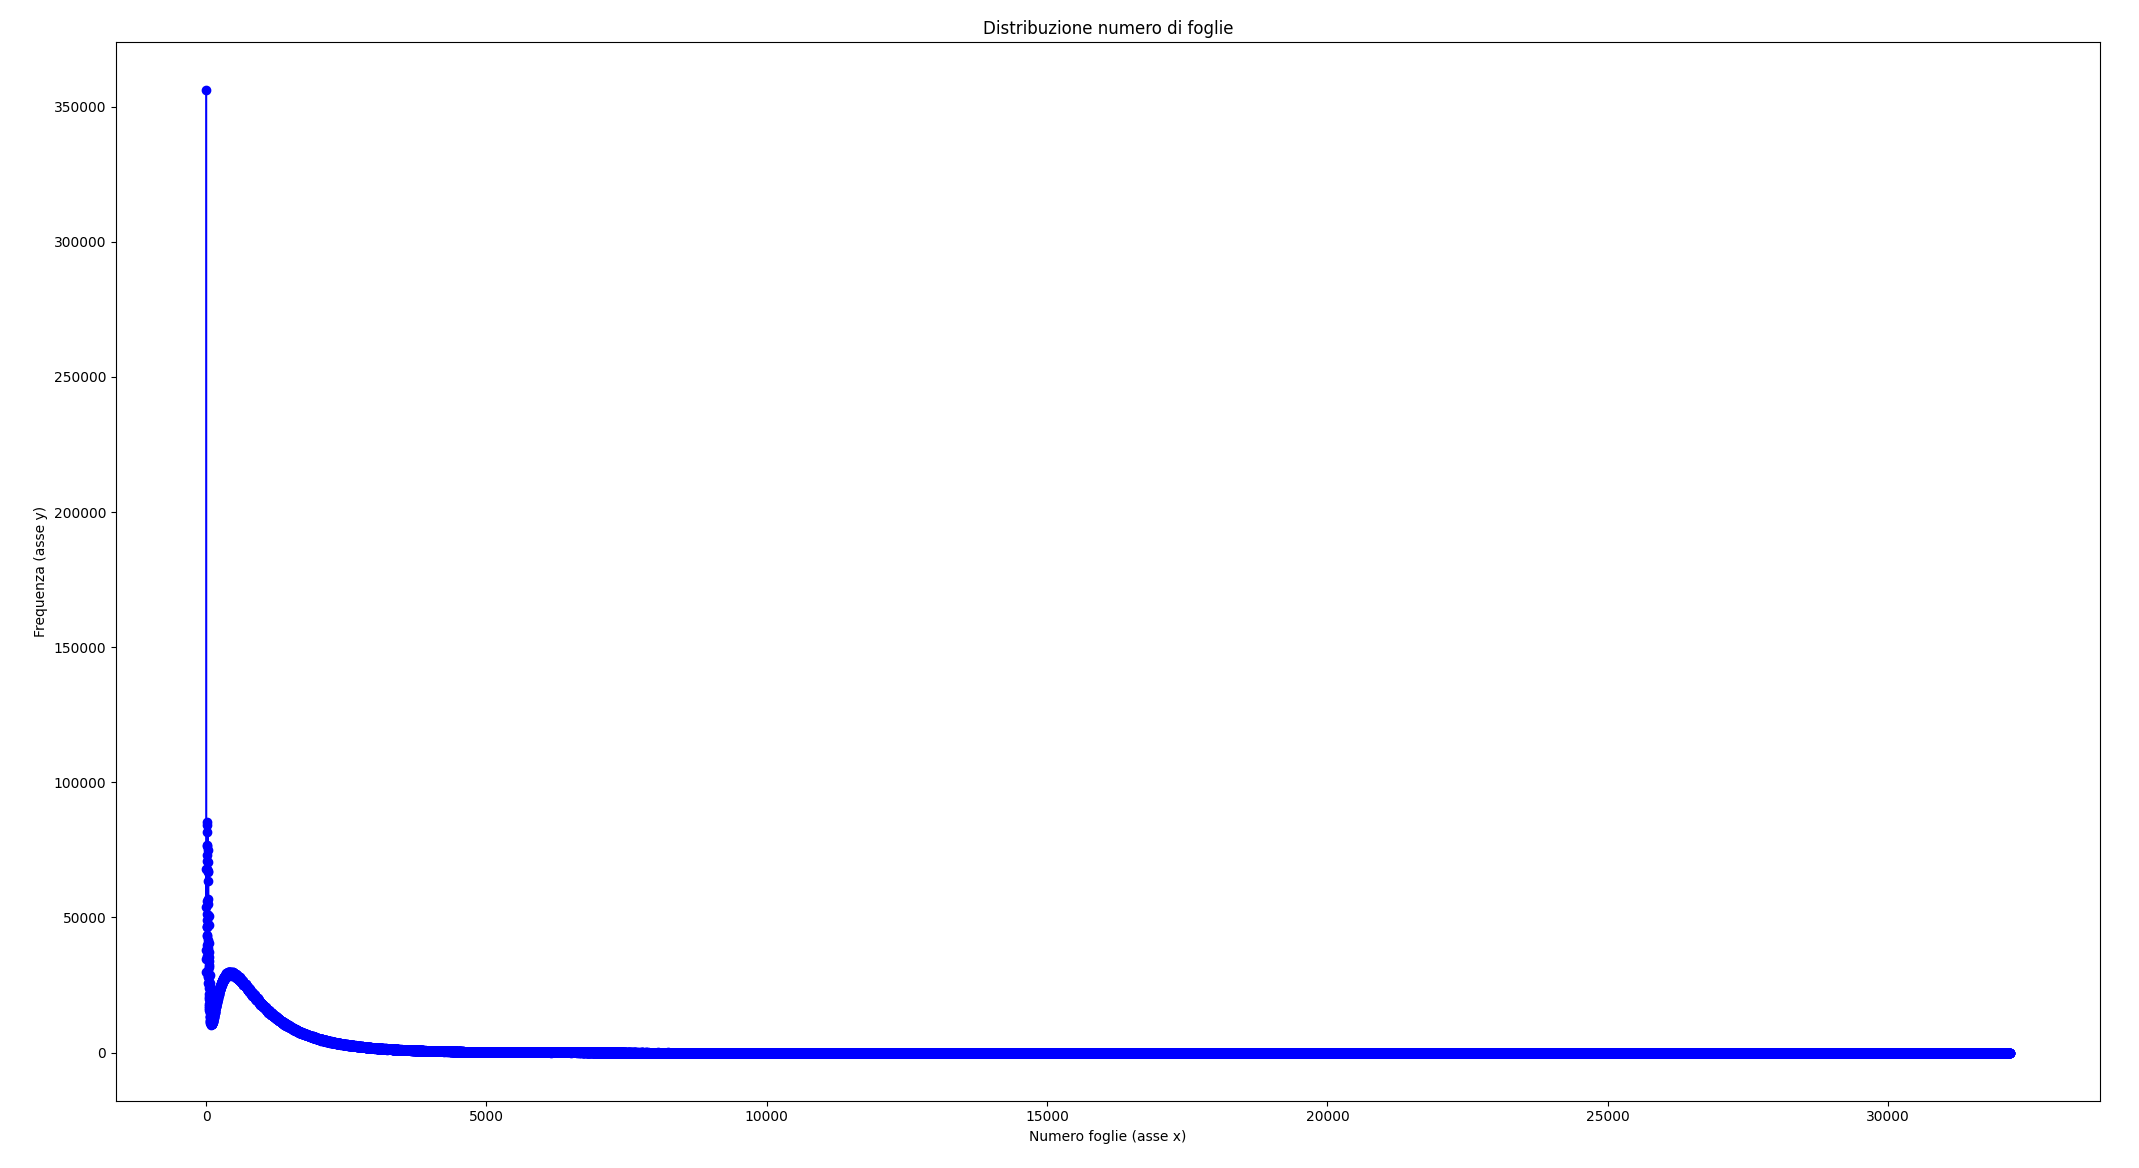
\includegraphics[width=1\textwidth]{imgs/grafico_base.png} % Specifica il percorso e il nome del file
    \caption{Grafico generale}
    \label{fig:etichetta}
\end{figure}

Si nota subito il picco sul valore 0, indicando che ci sono poco più di 356.142 partite con una sola foglia, corrispondenti approssimativamente a un 9\% del totale delle partite testate.

Queste sono partite banali, in cui si parte con una tessera doppia e poi nessuno dei due giocatori ha una seconda tessera che contenga il numero giocato come mossa iniziale.

\begin{figure}[h!]
    \centering
    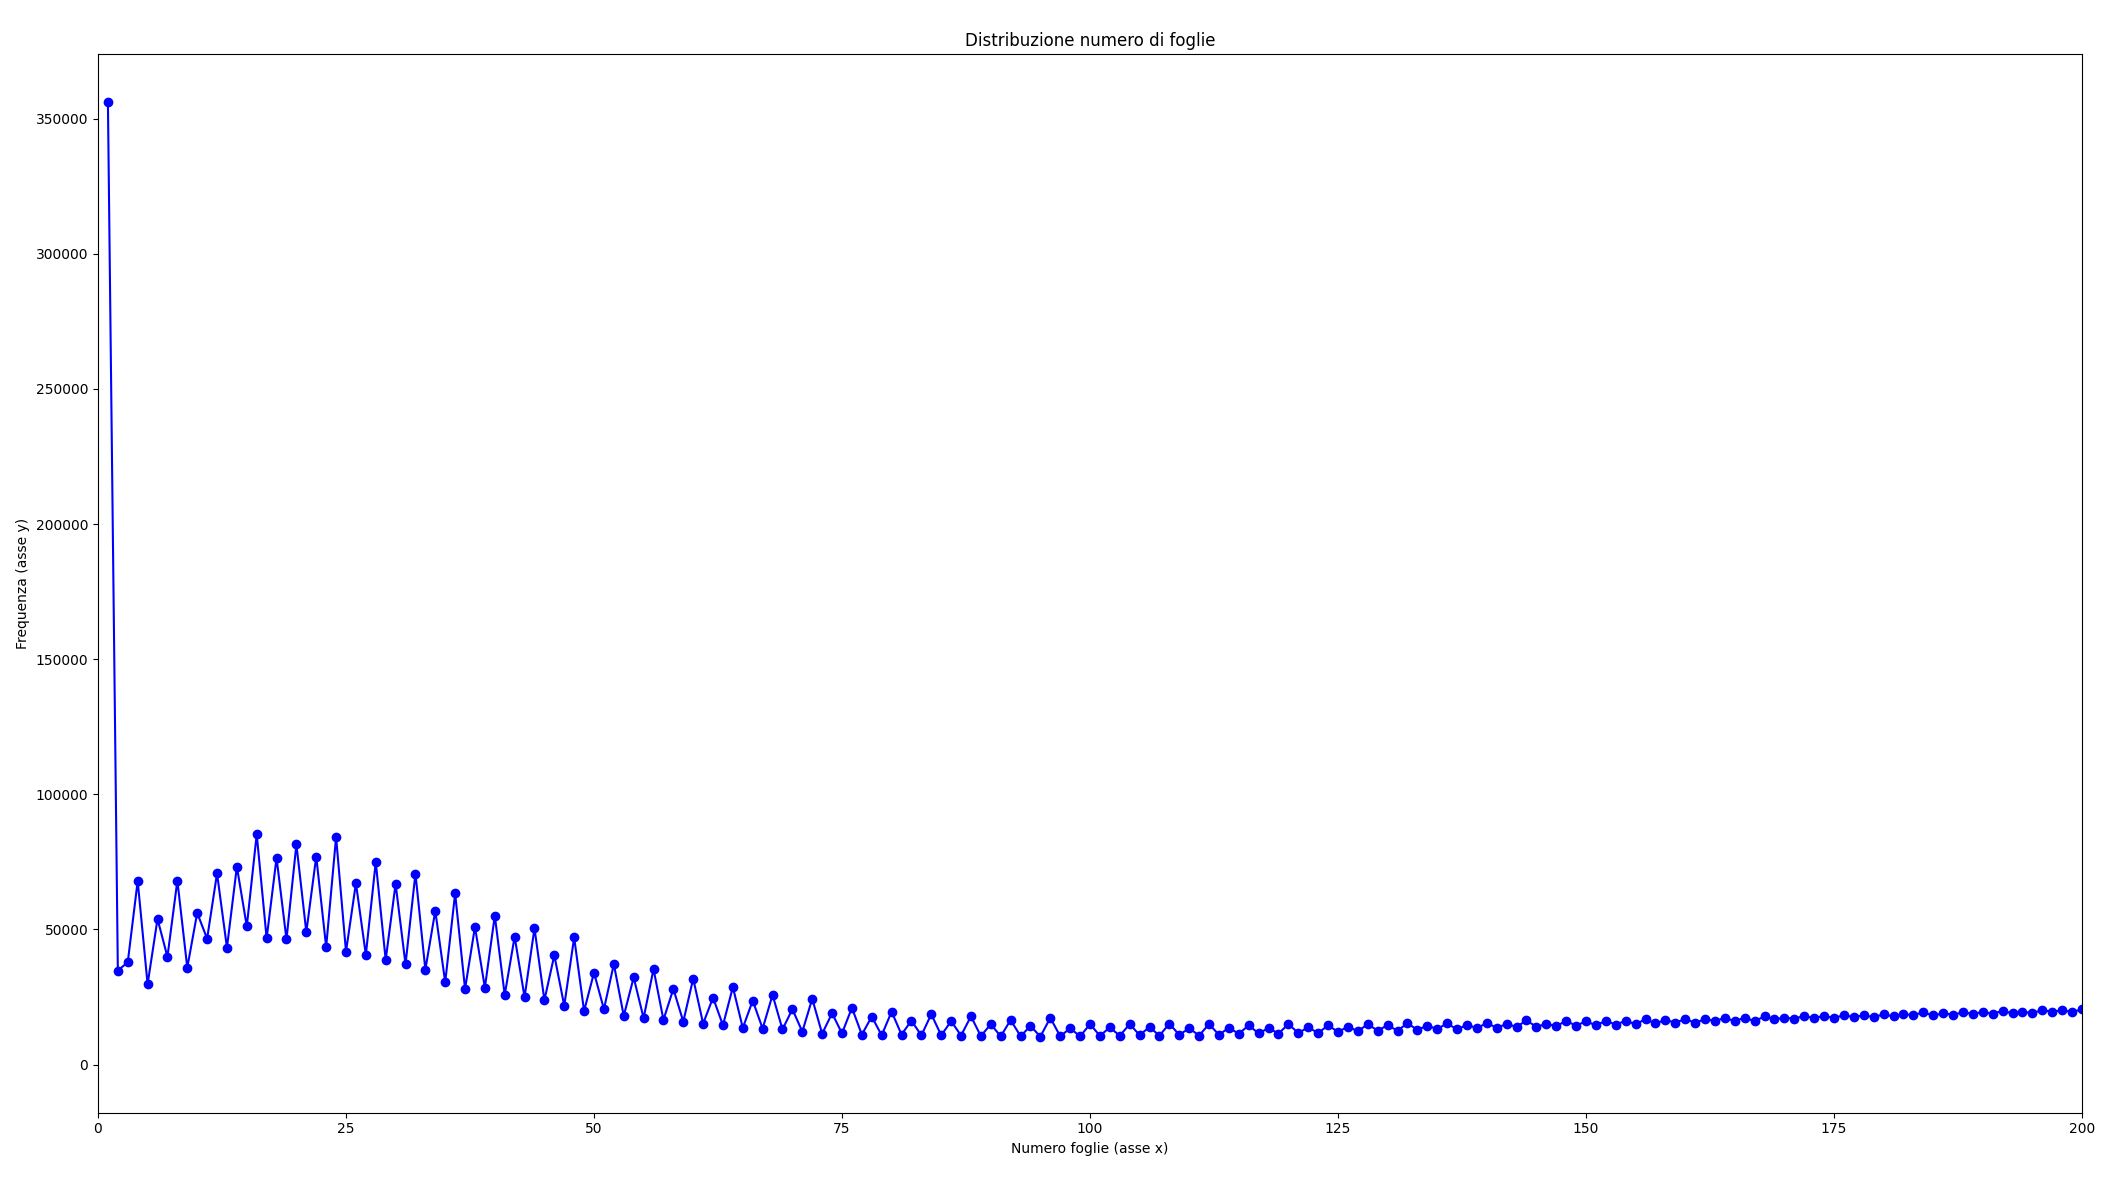
\includegraphics[width=1\textwidth]{imgs/grafico_0_200.png} % Specifica il percorso e il nome del file
    \caption{Ingrandimento dominio 0-200}
    \label{fig:etichetta}
\end{figure}

Curiosa l'alternanza dei valori, probabilmente solo una coincidenza che non porta a nulla di significativo.

\begin{figure}[h!]
    \centering
    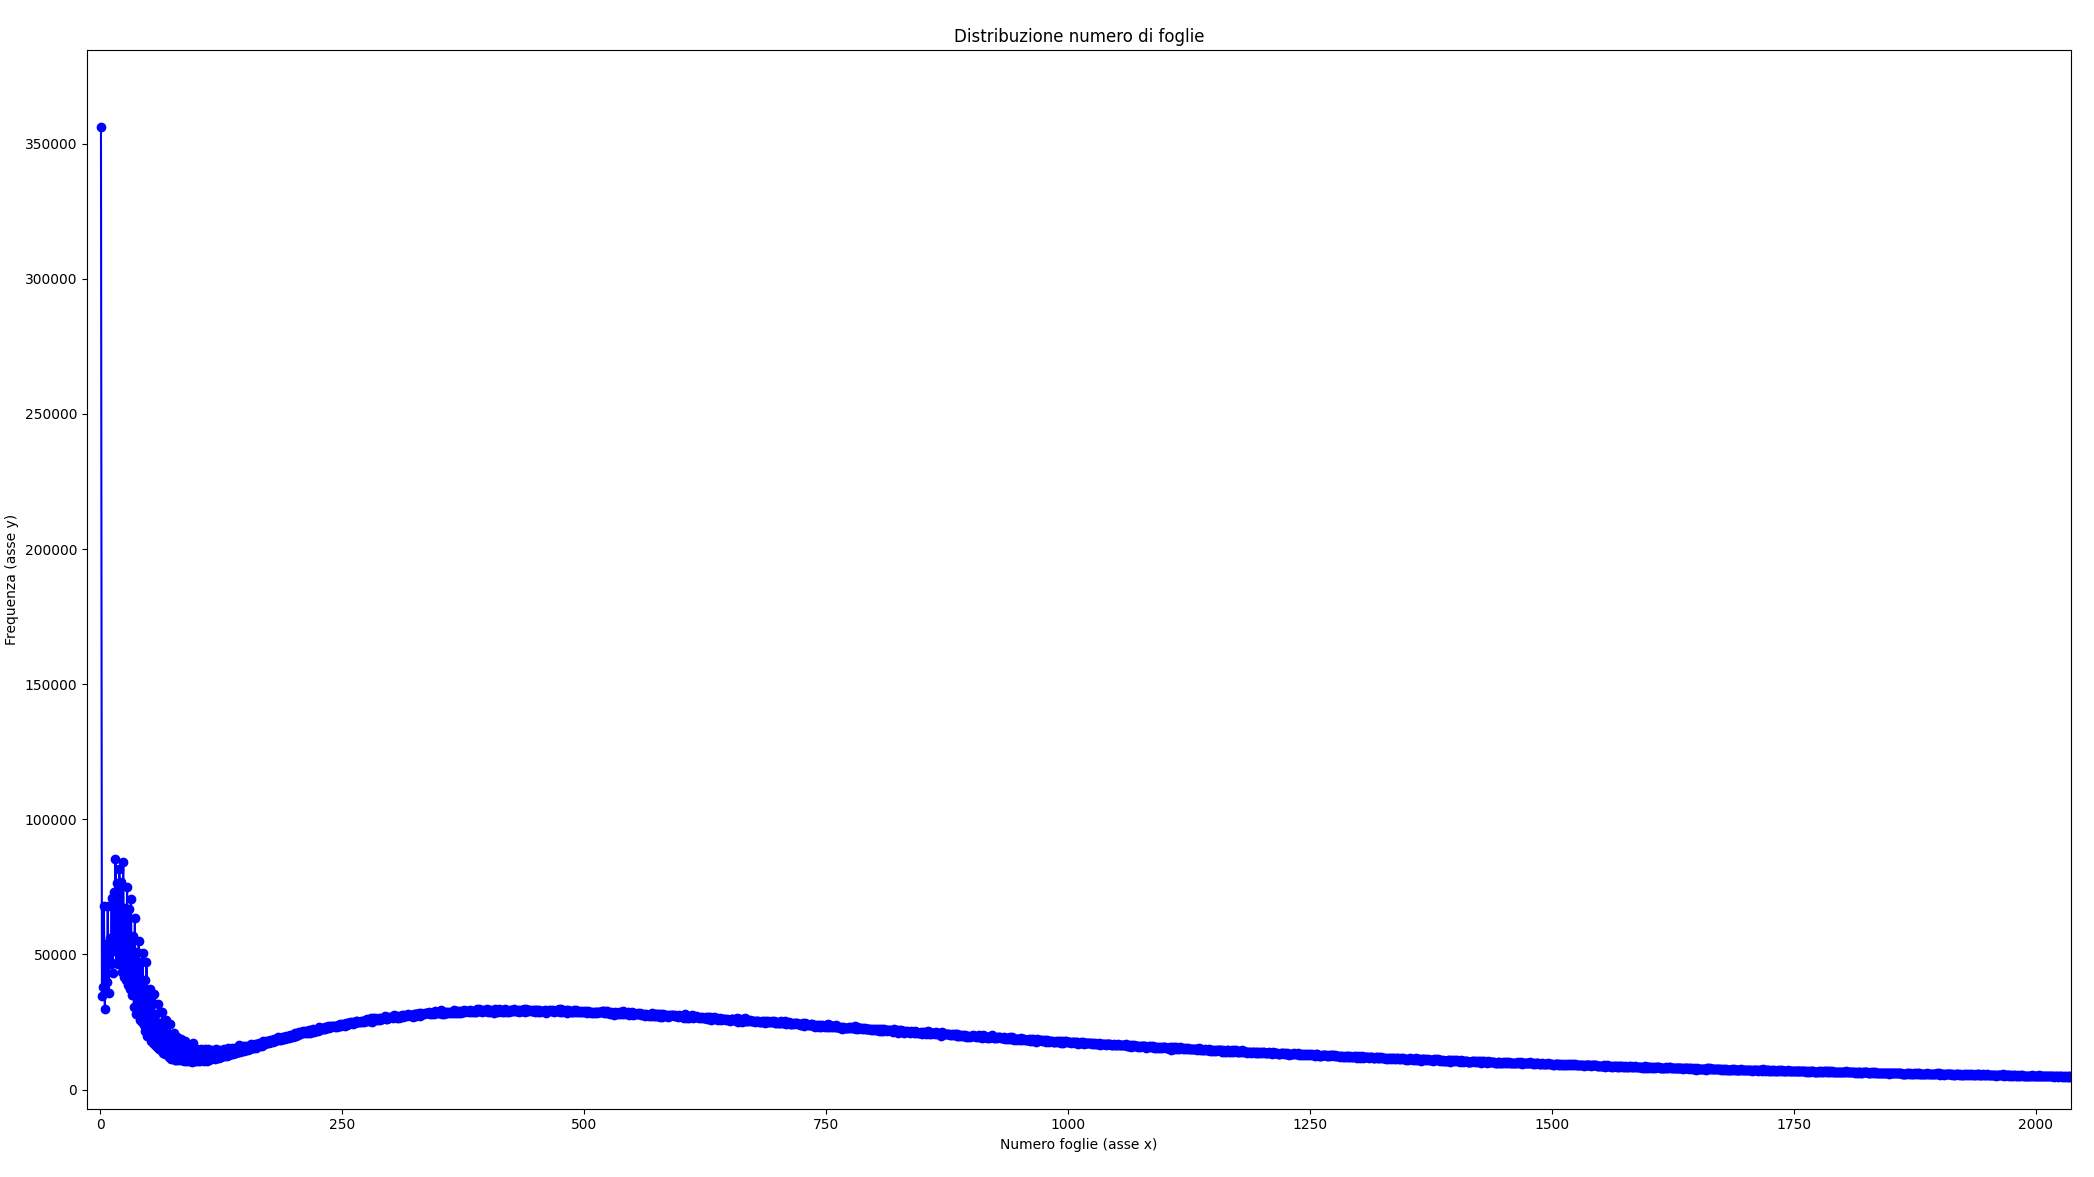
\includegraphics[width=1\textwidth]{imgs/grafico_0_2000.png} % Specifica il percorso e il nome del file
    \caption{Ingrandimento dominio 0-2000}
    \label{fig:etichetta}
\end{figure}

\begin{figure}[h!]
    \centering
    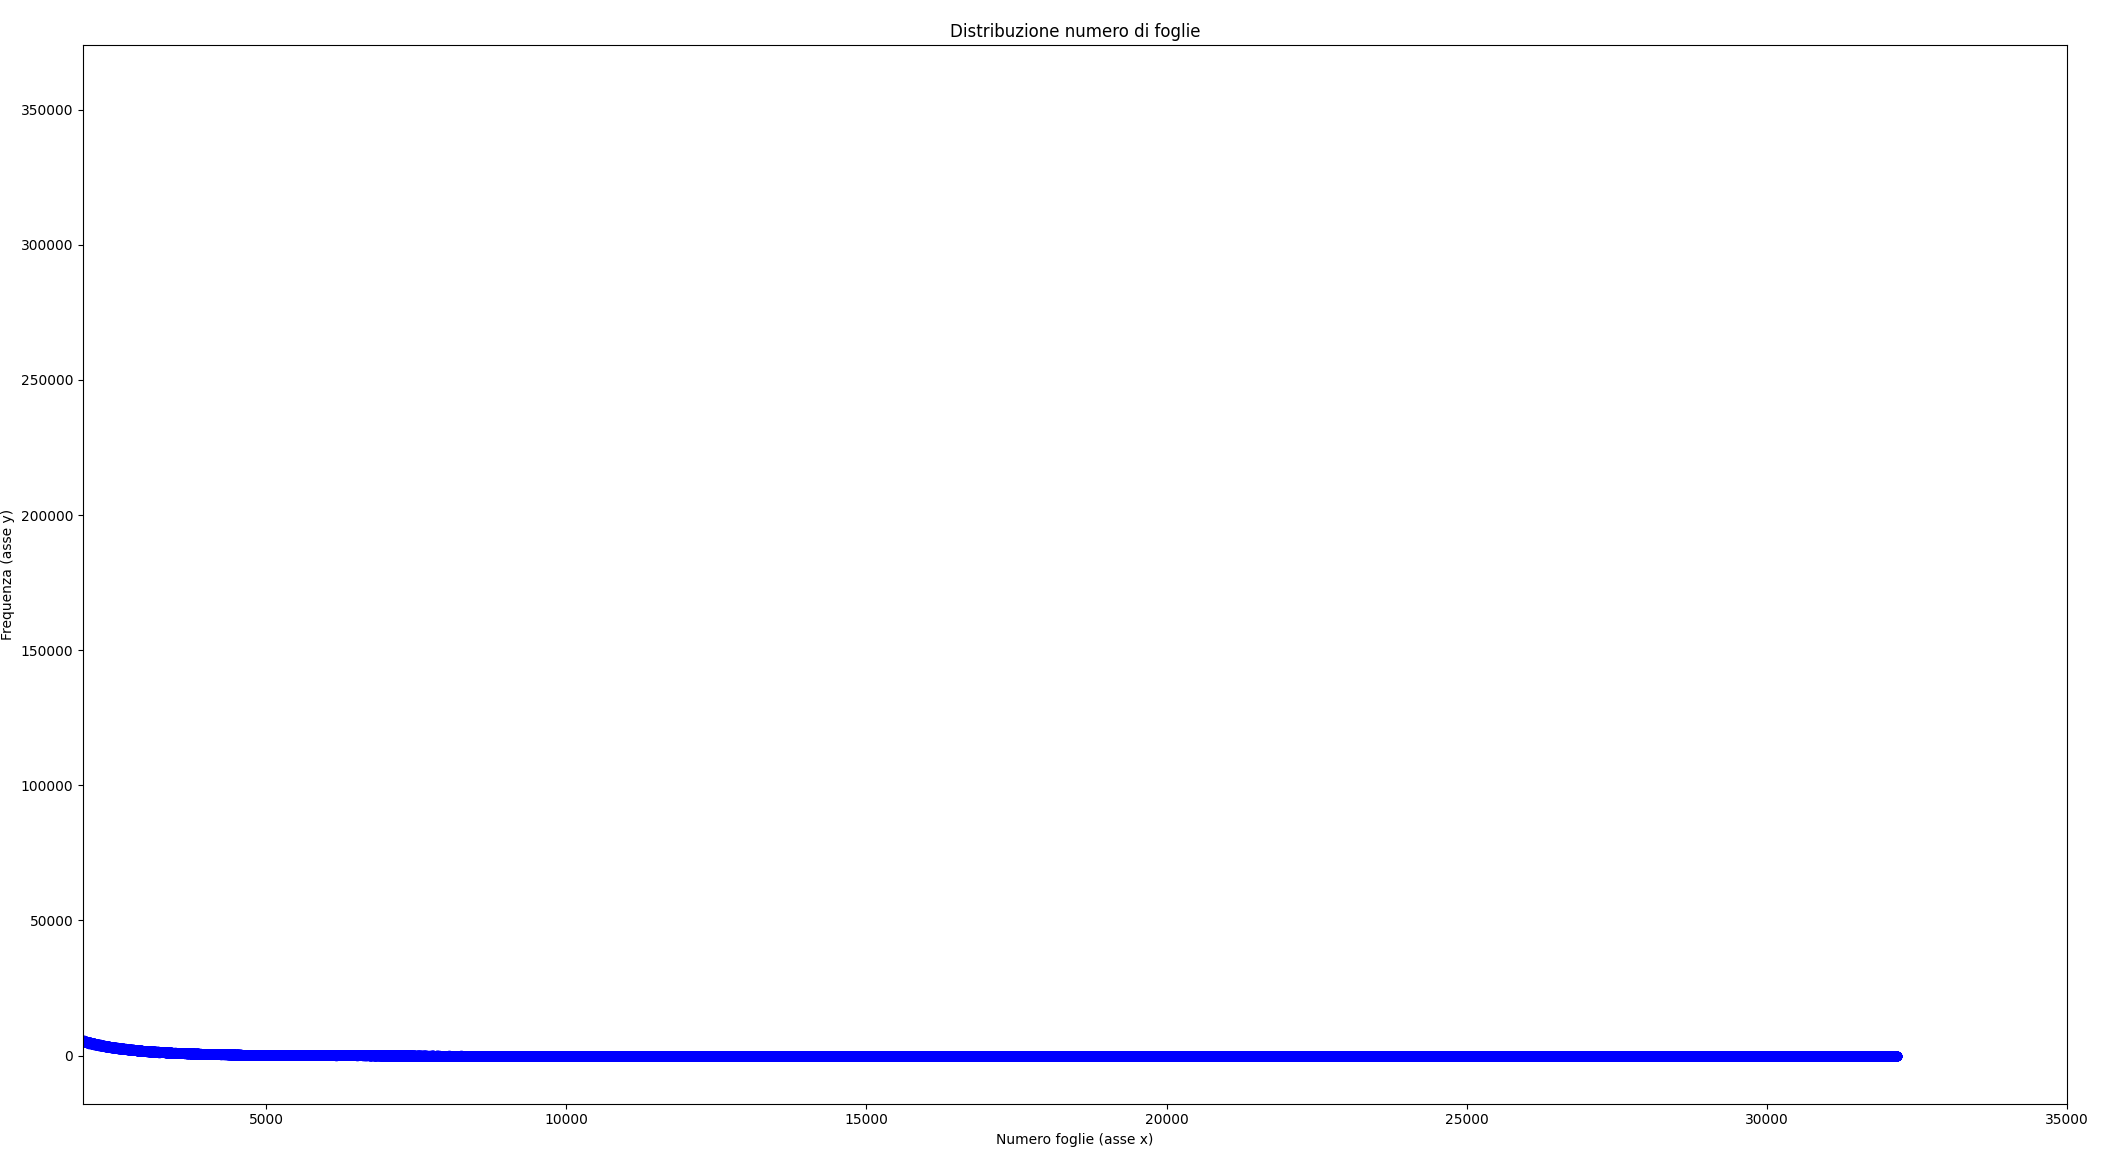
\includegraphics[width=1\textwidth]{imgs/grafico_2000_35000.png} % Specifica il percorso e il nome del file
    \caption{Ingrandimento dominio 2000-35000}
    \label{fig:etichetta}
\end{figure}




\chapter{Conclusioni}

Il set più forte trovato è sicuramente \(0|0, 0|1, 0|2, 0|3, 0|4, 0|5, 0|6\) che ha vinto la totalità delle 65 partite giocate.



\appendix
\chapter{Codice sorgente}
% Includi eventuali porzioni di codice

\bibliographystyle{plain} % Stile della bibliografia
\bibliography{bibliografia} % File .bib con riferimenti

\end{document}
